      Logo abaixo são apresentados os resultados da primeira iteração de avaliação do protótipo de alta fidelidade,
      seguindo o planejamento realizado.
      
      \begin{itemize}
       \item \textbf{Descrição e metodologia do roteiro da avaliação}
       
       \item \textbf{Comportamento dos usuários}
       
       Ao todo, os cinco usuários que avaliaram o protótipo conseguiram cumprir todas as tarefas estabelecidas 
       de todos os cenários. Agiram perante as atividades do protótipo de maneira intuitiva e não demoraram a 
       cumprir as funcionalidades dos cenários de avaliação estabelecidos.
       
       \item \textbf{Resumo das entrevistas}
       
       \item \textbf{Problemas de usabilidade identificados}
       
       \item \textbf{Paradas críticas}
       
       \item \textbf{Plano de correção}
      \end{itemize}
      
      Na figura \ref{asqalta} se encontram as respostas ao questionário ASQ pelos cinco usuários avaliados.
      
      \begin{figure}[!htb]
      \centering
      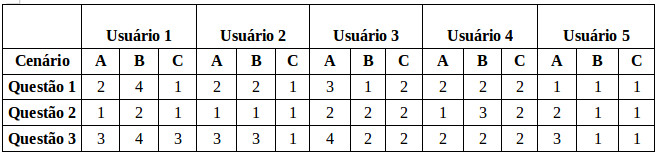
\includegraphics[scale=0.6]{figuras/asqalta.jpg}
      \caption{Resposta dos usuários ao questionário ASQ na primeira avaliação do protótipo de alta fidelidade}
      \label{asqalta}
      \end{figure}
      
      Na figura \ref{pssuqalta} se encontram as respostas ao questionário PSSUQ pelos cinco usuários avaliados.
      
      \begin{figure}[!htb]
      \centering
      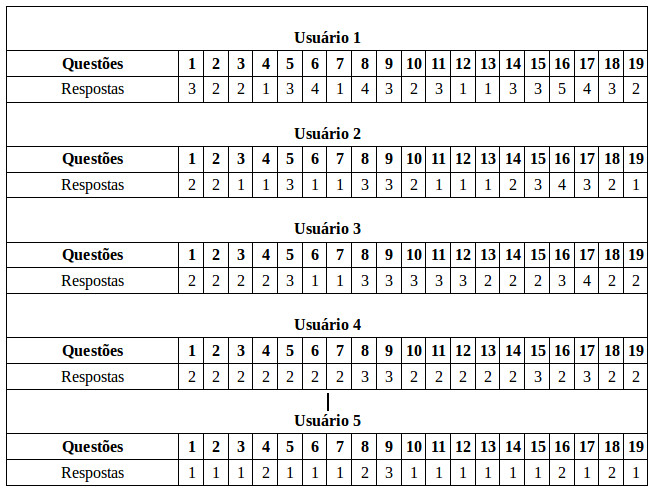
\includegraphics[scale=0.6]{figuras/pssuqalta.jpg}
      \caption{Resposta dos usuários ao questionário PSSUQ na primeira avaliação do protótipo de alta fidelidade}
      \label{pssuqalta}
      \end{figure}